\documentclass[12pt,a4paper]{report}

\usepackage[margin=1in]{geometry}
\usepackage{graphicx}
\usepackage{array}
\usepackage{booktabs}
\usepackage{float}
\usepackage{setspace}
\usepackage{titlesec}
\usepackage{tocloft}
\usepackage{enumitem}
\usepackage{hyperref}
\usepackage{xcolor}
\usepackage{url}

\hypersetup{
    colorlinks=true,
    linkcolor=black,
    urlcolor=blue,
    pdftitle={Internship Report},
    pdfauthor={KAMAL S}
}

\setstretch{1.3}
\setlength{\parindent}{0pt}
\setlength{\parskip}{0.6em}

\titleformat{\chapter}[display]
  {\bfseries\Large}
  {\chaptername~\thechapter}{10pt}{\Huge}

\begin{document}

% ── TITLE PAGE ───────────────────────────────────────────────────────────────
\begin{titlepage}
\centering

\includegraphics[height=2.5cm]{images/dept_logo_404257df.png}\par
\vspace{0.4cm}
{\Large VISVESVARAYA TECHNOLOGICAL UNIVERSITY\par}
\vspace{0.2cm}
{\large Jnana Sangama, Belagavi -- 590018\par}
\vspace{1cm}
{\Large An Internship Report\par}
\vspace{0.3cm}
{\large On\par}
\vspace{0.3cm}
{\Large \textquotedblleft FullStack developer\textquotedblright\par}
\vspace{0.3cm}
{\large Jan 27 to April 27\par}
\vspace{0.8cm}
Submitted in partial fulfillment of the requirements for the award of the degree of\par
\vspace{0.2cm}
{\Large Bachelor of Engineering\par}
\vspace{0.2cm}
in\par
\vspace{0.2cm}
{\Large Electronics and communications\par}
\vspace{0.8cm}
Submitted by\par
\vspace{0.2cm}
{\Large KAMAL S\par}
{\Large 1VI22EC066\par}
\vfill
{\Large DEPARTMENT OF ELECTRONICS AND COMMUNICATIONS\par}
{\Large VEMANA INSTITUTE OF TECHNOLOGY\par}
{\Large BENGALURU -- 560034\par}
\vspace{0.4cm}
{\Large 2025-2026\par}
\end{titlepage}

% ── CERTIFICATE PAGE ─────────────────────────────────────────────────────────
\pagenumbering{roman}
\setcounter{page}{1}
\begin{center}
{\Large Karnataka ReddyJana Sangha\par}
{\Large VEMANA INSTITUTE OF TECHNOLOGY\par}
(Affiliated to Visvesvaraya Technological University, Belagavi)\par
Koramangala, Bengaluru--560034\par
\vspace{0.5cm}
{\Large DEPARTMENT OF ELECTRONICS AND COMMUNICATIONS\par}
\vspace{0.8cm}
{\Large CERTIFICATE\par}
\end{center}

This is to certify that the internship entitled ``FullStack developer'' is a bonafide work carried out by KAMAL S (1VI22EC066) in partial fulfilment of the requirements for the award of Bachelor of Engineering degree in Electronics and communications, Visvesvaraya Technological University, Belagavi, during the academic year 2025-2026.

It is certified that all corrections and suggestions indicated for internal assessment have been duly incorporated in the report. The internship report has been approved as it satisfies the academic requirements prescribed for the said degree.

\vspace{1cm}
\begin{center}
\begin{tabular}{p{0.23\textwidth} p{0.23\textwidth} p{0.23\textwidth} p{0.23\textwidth}}
Internal Supervisor & External Supervisor & HOD & Principal \\
(Prof. Suma B V) & (Maneesh Kumar Varma) & (Dr. Suneeta) & (Dr. Vijayasimha Reddy B G) \\
\end{tabular}
\end{center}

\vspace{0.8cm}
Name of the Examiners\hfill Signature with Date\par
1.\par
2.\par

\newpage
\begin{center}
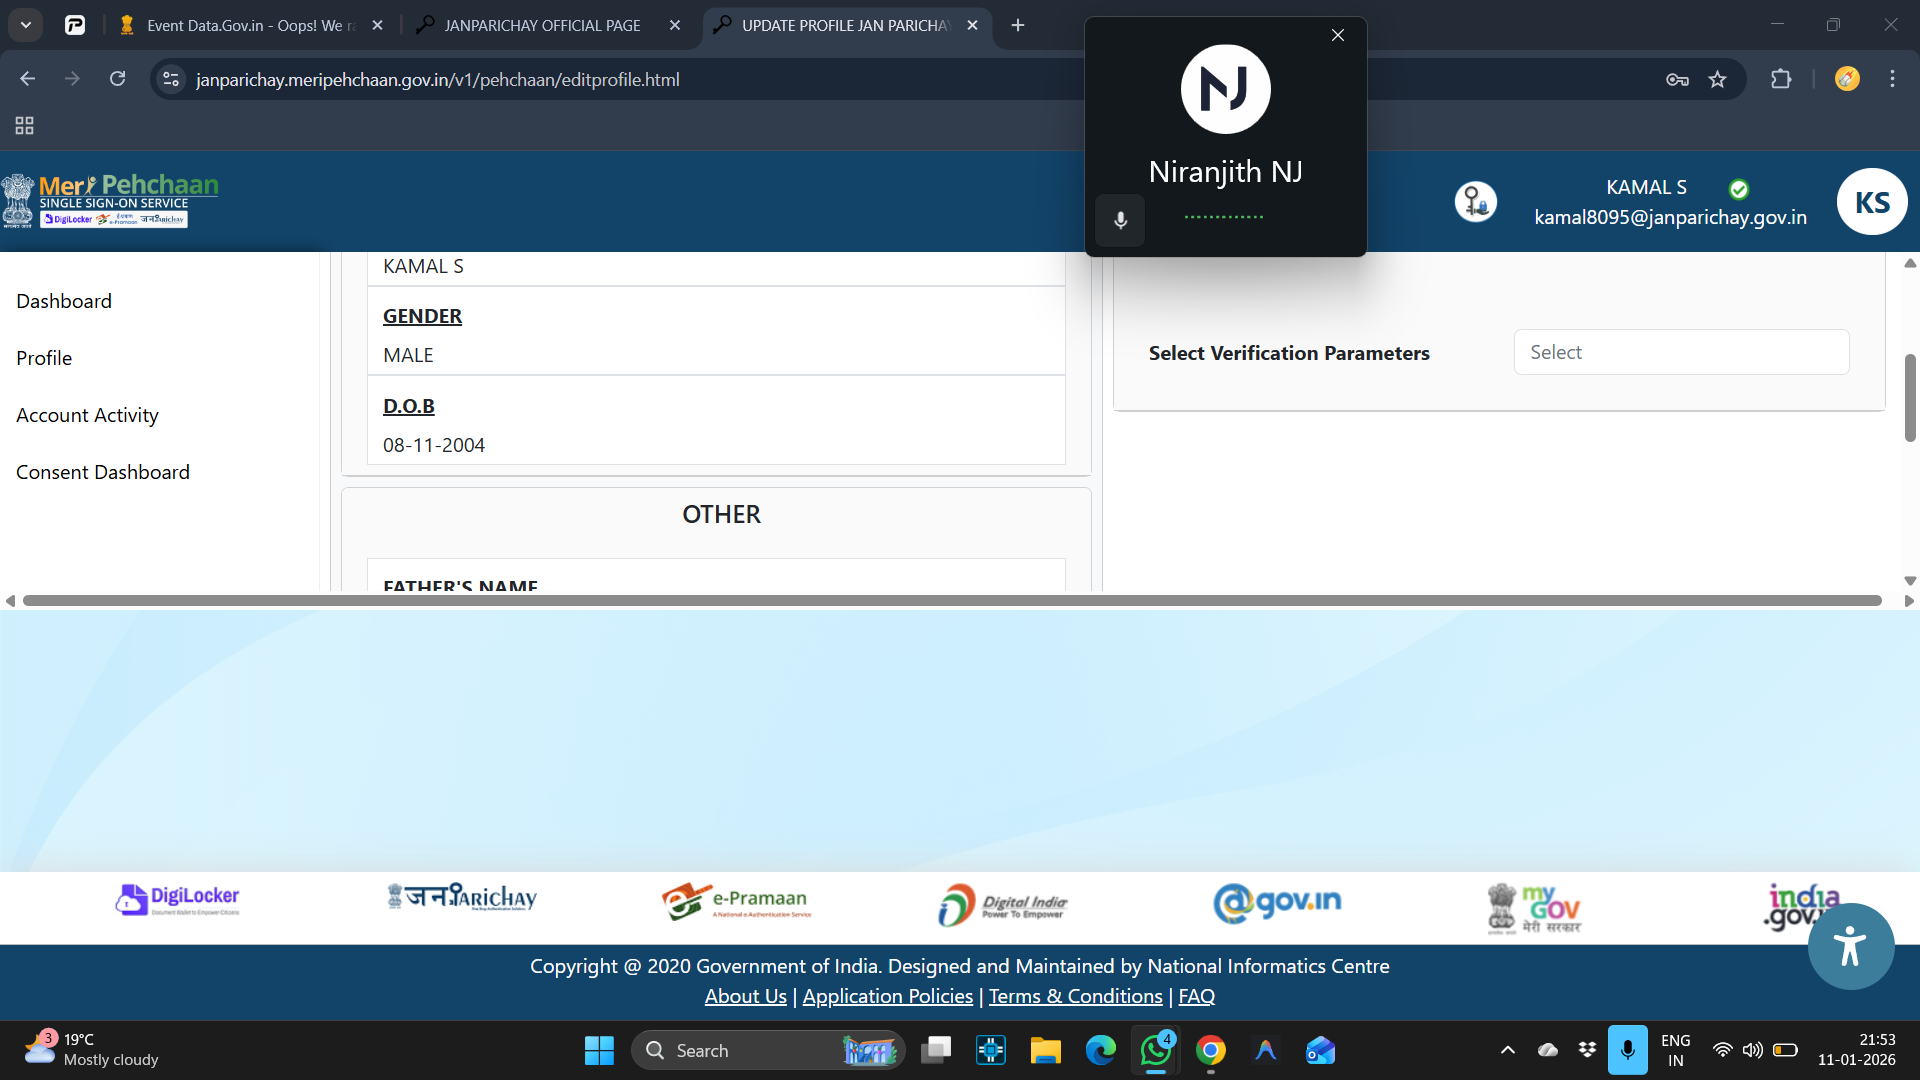
\includegraphics[width=0.9\textwidth]{images/cert_image_f8754fbf.png}
\end{center}


% ── ACKNOWLEDGEMENT ───────────────────────────────────────────────────────────
\newpage
\chapter*{ACKNOWLEDGEMENT}
\addcontentsline{toc}{chapter}{Acknowledgement}

I would like to express my sincere gratitude to Visvesvaraya Technological University (VTU) for providing me with the opportunity to undertake this internship as a part of my academic curriculum. I am thankful to our respected Principal, Dr. Vijayasimha Reddy B G, for his continuous support and encouragement throughout my academic journey.

I would like to extend my heartfelt thanks to the Head of the Department, Dr. Suneeta, for her guidance and support. I am especially grateful to my internal supervisor, Prof. Suma B V, for her valuable suggestions and continuous encouragement during the internship.

I would also like to thank my external supervisor, Mr. Maneesh Kumar Varma, at Supram Technologies, for providing me with the opportunity to work in a professional environment and for guiding me throughout the internship. I am deeply thankful to Supram Technologies for allowing me to gain hands-on experience and exposure to real-world engineering practices.

\vspace{0.5cm}
Kamal S\par
1VI22EC066\par

% ── ABSTRACT ─────────────────────────────────────────────────────────────────
\newpage
\chapter*{ABSTRACT}
\addcontentsline{toc}{chapter}{Abstract}

During my internship at Supram Technologies as a Full Stack Developer, I gained exposure to multiple domains including industrial UI design, embedded systems, middleware, and system-level development. Initially, I worked on designing web-based industrial dashboards and HMI interfaces, focusing on usability, clarity, and real-time data handling. This helped me understand how user interfaces are designed for industrial environments. I later explored embedded platforms such as Jetson Nano and Jetson Orin, along with ROS (Robot Operating System), to understand communication between different system modules. I also conducted research on IR and Ultrasonic sensors and prepared Gantt charts and technical budgets for project planning. In the next phase, I transitioned into full stack web development, where I worked on frontend-backend integration, API handling, and data flow management. Finally, I worked with Qualcomm tools for debugging, log analysis, and performance monitoring. This internship helped me gain practical knowledge of real-world system development and improved my technical and analytical skills.

% ── TABLE OF CONTENTS ─────────────────────────────────────────────────────────
\newpage
\tableofcontents
\addcontentsline{toc}{chapter}{Table of Contents}

\newpage
\listoffigures
\addcontentsline{toc}{chapter}{List of Figures}

% ── CHAPTER 1: INTRODUCTION ───────────────────────────────────────────────────
\pagenumbering{arabic}
\chapter{INTRODUCTION}

This chapter provides an introduction to my internship experience at Supram Technologies, where I worked as a Full Stack Developer. It outlines the objectives, scope, and relevance of the internship in relation to my academic background in Electronics and Communication Engineering. This chapter also discusses the evolution of technologies and current trends related to the work carried out during the internship.

\section{Internship Scope and Objectives}
The primary objective of my internship at Supram Technologies was to gain practical knowledge in real-world engineering and software development. The scope of the internship included working on industrial UI design, embedded platforms, middleware systems, and full stack web development. I aimed to understand system architecture, data flow, and integration between hardware and software components.

Additionally, the internship focused on developing problem-solving skills, improving technical documentation, and understanding project planning through tools like Gantt charts and budgeting. The scope also included exposure to Qualcomm development tools for debugging and performance analysis.

\section{Relevance of FullStack developer to Electronics and communications}
The role of a Full Stack Developer is highly relevant to Electronics and Communication Engineering as it involves system integration, data communication, and real-time processing. During the internship, I worked on technologies that connect hardware and software systems, which is a core concept in ECE.

Understanding embedded systems, ROS communication, and sensor integration helped me relate theoretical concepts such as signal processing, communication systems, and microcontrollers to real-world applications. Full stack development further enhanced my understanding of how data is processed, transmitted, and visualized.

\section{Evolution of Practices in the Field}
Over the years, engineering systems have evolved from simple standalone devices to complex interconnected systems. Earlier, systems were hardware-focused, but now they involve a combination of hardware, software, and networking. Technologies like embedded systems, IoT, and middleware have transformed how systems communicate and operate.

Full stack development has also evolved significantly, enabling developers to build complete applications from frontend to backend. This evolution has made system development more integrated and efficient.

\section{Current Trends and Technologies}
Current trends include the use of embedded AI platforms like Jetson Nano, middleware systems like ROS, and real-time data-driven applications. Full stack development using APIs and cloud-based systems is also widely used.

There is increasing focus on system integration, automation, and performance optimization. Tools like Qualcomm development platforms are used for advanced debugging and system analysis, making development more efficient.



% ── CHAPTER 2: ORGANISATION PROFILE ──────────────────────────────────────────
\chapter{ORGANISATION PROFILE}

Supram Technologies is an engineering-focused company that works on industrial solutions and advanced technology development. The company is involved in research, development, and implementation of systems across multiple domains including embedded systems, automation, and software development. During my internship, I had the opportunity to work in a professional environment and gain exposure to real-world engineering practices.

\section{Introduction}
Supram Technologies is a leading organization that provides structured learning, training, and internship programs to engineering students and professionals.


\begin{figure}[H]
\centering
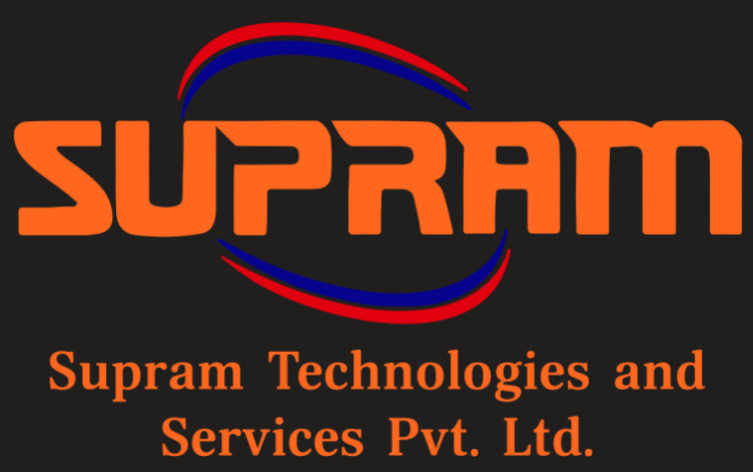
\includegraphics[width=0.45\textwidth]{images/company_logo_6e2c4cf1.png}
\caption{Supram Technologies Logo}
\end{figure}


\section{Vision and Mission of the Organization}
The vision of Supram Technologies is to deliver innovative engineering solutions that meet industrial standards and improve efficiency. The company aims to focus on research, development, and continuous improvement while maintaining high quality and reliability in its services.

\section{Programs and Services Offered}
Supram Technologies offers services in embedded systems development, industrial automation, and software solutions. The company focuses on integrating hardware and software systems for efficient performance.

They also work on system design, research, and development projects, providing solutions for real-world engineering problems.

\section{Organizational Impact and Reach}
Supram Technologies has contributed to industrial innovation by developing reliable and efficient engineering solutions. The company focuses on practical implementation and system optimization, making a significant impact in engineering and technology domains.

\section{Core Values}
\begin{itemize}[leftmargin=1.5em]
    \item Innovation
    \item Quality and Reliability
    \item Continuous Learning
    \item Technical Excellence
    \item Team Collaboration
\end{itemize}



% ── CHAPTER 3: WORK DONE / METHODOLOGY ────────────────────────────────────────
\chapter{WORK DONE / METHODOLOGY}

During my internship at Supram Technologies, I worked across multiple domains including UI design, embedded systems, middleware, and full stack development. Initially, I worked on designing industrial dashboards and HMI interfaces. Later, I explored embedded platforms and ROS communication.

I also worked on system planning, sensor research, and full stack web development. Finally, I used Qualcomm tools for debugging and performance analysis.

\section{Overview of Internship Work}
The internship at Supram Technologies provided structured exposure to the field of FullStack developer. The work involved hands-on application of domain knowledge in a professional setting.

\section{Tools and Technologies Used}
The tools and technologies used during the internship include Jetson Nano, Jetson Orin, ROS, GitHub, and Qualcomm development tools. I also worked with full stack technologies including frontend and backend development, API integration, and database handling.

\section{Work Process and Methodology}
The work process involved understanding requirements, researching technologies, designing system components, implementing solutions, and testing. Each phase was followed by review and optimization.

\section{Key Project and Case Study}
One of the key tasks was working on a full stack application:

\begin{itemize}[leftmargin=1.5em]
    \item Designed frontend interface
    \item Developed backend APIs
    \item Integrated frontend and backend
    \item Tested data flow and performance
\end{itemize}

This helped me understand complete system development.



\section{Challenges Faced}
Some challenges included understanding new technologies, debugging issues, and managing system integration. Learning multiple domains required continuous effort.

\section{Solutions Implemented}
These challenges were overcome by consistent learning, debugging, and guidance from mentors. Proper planning and testing helped improve system performance.



% ── CHAPTER 4: RESULTS AND DISCUSSION ────────────────────────────────────────
\chapter{RESULTS AND DISCUSSION}

This chapter discusses the results obtained during the internship and the learning outcomes achieved through various tasks.



\section{Outcomes of the Work}
The internship helped me gain practical knowledge in system development, full stack applications, and embedded systems. I was able to understand real-world engineering processes.

\section{Learning Outcomes}
I gained technical skills in full stack development, embedded systems, and debugging. I also improved problem-solving and communication skills.

\section{Analysis}
The internship provided valuable experience in real-world engineering. It helped me understand system design and integration effectively.



% ── CHAPTER 5: CONCLUSION ────────────────────────────────────────────────────
\chapter{CONCLUSION}

This chapter concludes the internship experience and summarizes the knowledge gained.



\section{Summary}
Overall, the internship at Supram Technologies was a valuable experience. It helped me understand multiple domains and improve my technical skills.

\section{Personal Growth}
The internship improved my confidence, problem-solving ability, and technical knowledge. It helped me grow professionally.

\section{Future Scope}
This internship opens opportunities in embedded systems, full stack development, and system engineering. It provides a strong foundation for my future career.

\end{document}
